\documentclass[psamsfonts]{amsart}

%-------Packages---------
\usepackage{amsmath}
\usepackage{amssymb}
\usepackage{amsfonts}
\usepackage{amsaddr}
\usepackage[all,arc]{xy}
\usepackage{enumerate}
\usepackage{mathrsfs}
\usepackage{physics}
\usepackage{bbm}
\usepackage{minted}
\usepackage{algorithm}
\usepackage{algpseudocode}
\usepackage{hyperref} 
\usepackage{mathtools}
\DeclarePairedDelimiter\floor{\lfloor}{\rfloor}
\usepackage{graphicx}
\graphicspath{ {./Figures/} }

%--------Theorem Environments--------
%theoremstyle{plain} --- default
\newtheorem{thm}{Theorem}[section]
\newtheorem{cor}[thm]{Corollary}
\newtheorem{prop}[thm]{Proposition}
\newtheorem{lem}[thm]{Lemma}
\newtheorem{conj}[thm]{Conjecture}
\newtheorem{quest}[thm]{Question}

\theoremstyle{definition}
\newtheorem{defn}[thm]{Definition}
\newtheorem{defns}[thm]{Definitions}
\newtheorem{con}[thm]{Construction}
\newtheorem{exmp}[thm]{Example}
\newtheorem{exmps}[thm]{Examples}
\newtheorem{notn}[thm]{Notation}
\newtheorem{notns}[thm]{Notations}
\newtheorem{addm}[thm]{Addendum}
\newtheorem{exer}[thm]{Exercise}

\theoremstyle{remark}
\newtheorem{rem}[thm]{Remark}
\newtheorem{rems}[thm]{Remarks}
\newtheorem{warn}[thm]{Warning}
\newtheorem{sch}[thm]{Scholium}

\makeatletter
\let\c@equation\c@thm
\makeatother
\numberwithin{equation}{section}

\bibliographystyle{plain}

\begin{document}

%--------Meta Data: Fill in your info------
\title{Contagion on Classical Random Graphs}

\author{Lucas H. McCabe}

\address{Whiting School of Engineering, Johns Hopkins University}

\email{lucas.mccabe@jhu.edu}

\date{\today}

\begin{abstract}

The emergence of complex systems science has inspired efforts to understand stochastic processes in networks. Beginning with first principles, we leverage analytical and computational methods to derive properties of contact processes on classical random graphs and provide a Python library for corresponding empirical simulations. Finally, we present a search and simulation approach to estimating outbreak-regulating vaccine rollout rates within our random graph framework. Our observations and inferences give rise to epidemiological, economic, and public policy opportunities for future research.
\end{abstract}

\maketitle

\tableofcontents

\section{Problem Setup and Exposition}

We model a simple social network with a classical random graph $G(n, p_{adj})$, consisting of n nodes, whereby any two nodes are connected with probability $p_{adj}$. One randomly-selected node is infected with a virus $V(p_{inf}, \tau)$, becoming Patient Zero. During a time step, each infected node spreads the virus to each of its connected nodes with probability $p_{inf}$.  The expected number of time steps for a node to recover from infection is $\tau$. For mathematical convenience, we ignore vital dynamics and assume that there are no births or deaths in the network.

Our primary aim is to develop analytical insights from first principles to better-understand contact processes in classical random graphs. Where tractable, we derive results in our random graph framework that correspond to results found using traditional epidemiological approaches. Where analytical solutions are less practical, we rely on computation and simulation approaches.

\section{Modeling Recovery}

We model the recovery process for a single infected node as a sequence of Bernoulli trials with success probability $p_{rec}$ occurring at each time step, with the success of a trial indicating a node's recovery from infection. So $p_{rec}$, the probability an infected node recovers in a given time step, is the value of $p$ for which $\sum_{k=1}^{\infty} (1 - p)^{k-1}p = \tau$. 

This means that $p_{rec}$ is equivalent to the maximum likelihood estimate of $p$ for a geometric random variable with expectation $\mathbb{E}[Geometric(p)] = \tau$, leaving $p_{rec} = \frac{1}{\tau}$.

\section{Calculating Basic Reproduction Number}

Of interest to epidemiologists and policymakers is a disease's basic reproduction number, which is the expected number of infections generated by one infected individual in a population of susceptible individuals. We present a method of computing the basic reproduction number of a virus $V(p_{inf}, \tau)$ on a random graph $G(n, p_{adj})$.

We begin by assuming no innate immunity. The event ${F_{XY}}$ that some node $X$ infected at time step zero (Patient Zero) and transmits the virus to some node $Y$ in time step one has probability $P(F_{XY}) = p_{adj} \cdot  p_{inf}$. On the other hand, the event ${F_{XY, t}}$, that Patient Zero transmits the virus to node Y by time step $t$ has probability:

\begin{align}
P(F_{XY, t}) &= \sum_{k=0}^{t} p_{adj} \cdot  p_{inf} \cdot P(\text{node $X$ is infected at step $k$}) \nonumber\\
&=\sum_{k=0}^{t} p_{adj} \cdot  p_{inf} \cdot (1 -p_{rec})^k \nonumber\\
&=\sum_{k=0}^{t} p_{adj} \cdot  p_{inf} \cdot \Big(1 -\frac{1}{\tau}\Big)^k \nonumber\\
&= p_{adj} \cdot  p_{inf} \cdot \sum_{k=0}^{t} \Big(1 -\frac{1}{\tau}\Big)^k
\end{align}

From here, we may calculate a basic reproduction number for $V(p_{inf}, \tau)$ on $G(n, p_{adj})$:

\begin{align}
R_0 &= (n-1) \lim_{t \to \infty} P(F_{XY, t}) \nonumber\\
&= (n-1) \lim_{t \to \infty} \Bigg(p_{adj} \cdot  p_{inf} \cdot \sum_{k=0}^{t} \Big(1 -\frac{1}{\tau}\Big)^k\Bigg) \nonumber
\end{align}

Since this is a geometric series with start term $(n-1)  p_{adj} p_{inf}$ and common ratio $1 -\frac{1}{\tau}$:

\begin{align}
R_0 &= (n-1) \frac{p_{adj} \cdot  p_{inf}}{1-(1 -\frac{1}{\tau})} \nonumber\\
&= (n-1) \frac{p_{adj} \cdot  p_{inf}}{\frac{1}{\tau}} \nonumber\\
&= (n-1) \cdot p_{adj} \cdot  p_{inf} \cdot \tau
\end{align}

which is equivalent to the usual $R_0 = \beta \tau$ formulation from compartamental epidemiology, where $\beta = (n-1) p_{adj}  p_{inf}$ is the initial number of infection-inducing contacts per unit time.

\section{A Random Graph SIS Model}

Let $I(t)$ represent the expected number of infections at time step $t$, and let $S(t)$ expected represent the number of susceptible individuals at time step $t$. We assume no interventions, such as behavioral changes or clinical treatments, are anticipated.

\begin{align}
I(t+1) &= I(t) + [\text{new infections}] - [\text{new recoveries}] \nonumber\\
&= I(t) + \sum_{k=1}^{I(t)} \sum_{j=1}^{S(t)} P(F_{kY}) - I(t)p_{rec} \nonumber\\
&= I(t) + I(t)S(t)P(F_{XY}) - I(t)\frac{1}{\tau} \nonumber\\
&= I(t)\Bigg[1 + S(t)P(F_{XY}) - \frac{1}{\tau}\Bigg]
\end{align}

In the susceptible-infected-susceptible (SIS) model, recovered individuals may become susceptible again. This model is relevant for illnesses such as the common cold, which confers no durable immunity after recovery.  In this case:

\begin{equation}
I_{SIS}(t+1) = I_{SIS}(t)\Bigg[1 + \Big(n-I_{SIS}(t)\Big)p_{adj} \cdot p_{inf} - \frac{1}{\tau}\Bigg]
\end{equation}

which is a concave-down parabola with derivative

\begin{equation}
\pdv{I_{SIS}(t+1)}{I_{SIS}(t)} = p_{adj} \cdot p_{inf} \cdot \Big(n-2 I_{SIS}(t)\Big) + \Big(1 - \frac{1}{\tau}\Big) \nonumber
\end{equation}

The expected maximum infected population size, $M_{SIS}(n, p_{adj}, p_{inf}, \tau)$, is found at the inflection point of (4.2), where:

\begin{equation}
M_{SIS}(n, p_{adj}, p_{inf}, \tau) = \frac{1}{2}\Big[n + \frac{\tau - 1}{\tau p_{adj}p_{inf}}\Big]
\end{equation}

If $M_{SIS}(n, p_{adj}, p_{inf}, \tau) \geq n$, then the number of infected individuals is bounded only by the size of the graph, and the full population is infected before the outbreak is under control. This is undesirable.

If, on the other hand, $R_0 > \frac{n-1}{n}(\tau - 1)$, then we can expect the outbreak to taper off before the full population is infected. In the thermodynamic limit, this threshold simplifies to $R_0 > \tau - 1$ and suggests that even an aggressive infection may be contained if the expected time to recover is sufficiently brief.

\section{A Random Graph SIR Model}

In the susceptible-infected-recovered model, infected individuals achieve immunity when they recover and are no longer susceptible. Let $R(t)$ represent the expected number of recovered individuals at time step $t$. (4.1) remains valid, but now $S_{SIR}(t) = n - I_{SIR}(t) - R(t)$. As such:

\begin{equation}
I_{SIR}(t+1) = I_{SIR}(t)\Bigg[1 + \Big(n - I_{SIR}(t) - R(t)\Big)p_{adj} \cdot p_{inf} -  \frac{1}{\tau}\Bigg] \text{, with}
\end{equation}
\begin{equation}
R(t+1) = R(t) + \frac{I_{SIR}(t)}{\tau} \text{,} \nonumber
\end{equation}
\begin{equation}
I_{SIR}(0)=1 \text{, and} \nonumber
\end{equation}
\begin{equation}
R(0)=0 \nonumber
\end{equation}

which reduces to:

\begin{equation}
I_{SIR}(t+1) = I_{SIR}(t)\Bigg[1 + \Big(n - I_{SIR}(t) - \frac{1}{\tau} \sum_{k=0}^{t-1}I_{SIR}(k)\Big)p_{adj} \cdot p_{inf} -  \frac{1}{\tau}\Bigg] \text{, with}
\end{equation}
\begin{equation}
I_{SIR}(t | t\leq0)=1 \nonumber
\end{equation}

or

\begin{equation}
I_{SIR}(t+1) = \prod_{k=0}^t\Bigg[1 + \Big(n - I_{SIR}(t) - \frac{1}{\tau} \sum_{j=0}^{t-1}I_{SIR}(j)\Big)p_{adj} \cdot p_{inf} -  \frac{1}{\tau}\Bigg] \text{, with}
\end{equation}
\begin{equation}
I_{SIR}(t | t\leq0)=1 \nonumber
\end{equation}

Exact solutions of these equations may be analytically intractable, but they can be quickly evaluated with a pair of recursive functions, exhibited in \textit{Supplemental: Sample Code for $estimate\_I$} and \textit{Supplemental: Sample Code for $estimate\_R$}.

Of note, however, is that (5.1) implies that the infected population grows until $\Bigg[\Big(n - I_{SIR}(t) - R(t)\Big)p_{adj} \cdot p_{inf}\Bigg] \leq \frac{1}{\tau}$, which occus when $S_{SIR}(t) \leq \frac{n-1}{R_0}$ or $\Big(\frac{S_{SIR}(t)}{n}\Big)\leq \frac{n-1}{nR_0}$. In the thermodynamic limit, this is:

\begin{equation}
\Big(\frac{S_{SIR}(t)}{n}\Big)R_0 \leq 1
\end{equation}

representing the illness's endemic steady state.

From the endemic steady state, we conclude that the fraction of the population not susceptible to the disease must be at least $1 - \frac{1}{R_0}$, which is identical to the usual expression for herd immunity we see in dynamical models.

\section{Vaccinations in the Random Graph SIR Model}

Let us consider a vaccine that is effective against transmission with uniform probability $\phi$ and is administered to the population with uniform probability $\omega$ at time step 0. Again, (4.1) remains valid, but now $P(F_{kY}) = p_{adj}p_{inf}(1-\omega\phi)$. We note that administering a vaccine in this manner is equivalent to simply scaling the edge probability $p_{adj}$ by a factor of $(1-\omega\phi)$. So:

\begin{equation}
I_{SIR}(t+1) = I_{SIR}(t)\Bigg[1 + \Big(n - I_{SIR}(t) - R(t)\Big)p_{adj} \cdot p_{inf}(1-\omega\phi) -  \frac{1}{\tau}\Bigg] \text{, with}
\end{equation}
\begin{equation}
R(t+1) = R(t) + \frac{I_{SIR}(t)}{\tau} \text{,} \nonumber
\end{equation}
\begin{equation}
I_{SIR}(0)=1 \text{, and} \nonumber
\end{equation}
\begin{equation}
R(0)=0 \nonumber
\end{equation}

which is increasing until 

\begin{equation}
S_{SIR}(t) \leq \frac{n-1}{R_0 (1-\omega\phi)} 
\end{equation}

But this is only the case if the vaccination is administered at the onset of the epidemic and the vaccine prevalence remains constant. More realistically, the vaccine has a gradual rollout.

We consider a linear rollout. The rollout may have a delay of $d$ time steps, a period during which vaccine prevalence is zero. The rollout strategy does not affect the effectiveness of the vaccine at an individual level, so $\phi$ remains constant. We represent the rollout as a piecewise vaccine prevalence function:

\begin{equation}
\omega(t) = 
	\begin{cases}
		0 & \text{if $t \leq d$} \\
		\alpha(t-d) & \text{if $d < t \leq d + \frac{1}{\alpha}$} \\
		1 & \text{otherwise}
	\end{cases}
\end{equation}

where the coefficient $\alpha \in (0, 1]$ is a parameter describing the rate of the rollout. With a gradual linear rollout, (6.1) is modified slightly:

\begin{equation}
I_{SIR}(t+1) = I_{SIR}(t)\Bigg[1 + \Big(n - I_{SIR}(t) - R(t)\Big)p_{adj} \cdot p_{inf}(1-\omega(t) \phi) -  \frac{1}{\tau}\Bigg] \text{, with}
\end{equation}
\begin{equation}
R(t+1) = R(t) + \frac{I_{SIR}(t)}{\tau} \text{,} \nonumber
\end{equation}
\begin{equation}
I_{SIR}(0)=1 \text{, and} \nonumber
\end{equation}
\begin{equation}
R(0)=0 \nonumber
\end{equation}

Likewise, (6.2) is modified slightly to account for the rollout, whereby (6.4) increases until:

\begin{equation}
S_{SIR}(t) \leq 
	\begin{cases}
		\frac{n-1}{R_0}  & \text{if $t \leq d$} \\
		\frac{n-1}{R_0 (1-\alpha(t-d)\phi)}  & \text{if $d < t \leq d + \frac{1}{\alpha}$} \\
		\frac{n-1}{R_0 (1-\phi)}  & \text{otherwise}
	\end{cases}
\end{equation}

noting that the uniform vaccine prevalence model of (6.1) and (6.2) is achieved from (6.4) and (6.5) by simply selecting $\alpha = 1$ and $d=0$.

\section{Vaccination Rollout Strategy in the Random Graph SIR Model}

Assuming that planners, such as government officials, are operating in good faith, the rollout begins as soon as a vaccine is available, and thus $d$ is determined by the vaccine development process, as is $\phi$. Realistically, $\alpha$ is the only manipulatable variable for planners when implementing a vaccine rollout. 

To simulate implementations of the random graph SIR model described in Sections 5 and 6, we provide a Python library, available on GitHub \href{https://github.com/lucasmccabe/Epidemics-on-Random-Graphs}{here}. The main classes are exhibited in \textit{Supplemental: Sample Code for the Virus Class}, \textit{Supplemental: Sample Code for the Vaccine Class}, and \textit{Supplemental: Sample Code for the Experiment Class}, but additional relevant information can be found in the GitHub repository.

Explicit thresholds for $\alpha$ may be intractable to derive analytically. Luckily, $\alpha$ is explicitly bounded by the range $(0, 1]$, making estimation of $\alpha$ threshold values particularly tractable by search and simulation approaches. Using our simulation library, we implement a binary search method for estimating a lower bound for $\alpha$ that leads to an outbreak's endemic steady state. Pseudocode for this method is shown in Algorithm \ref{alg1}. Sample code for our algorithm is provided in \textit{Supplemental: Sample Code for \textit{estimate\_alpha}}.

For demonstration, we show an example of this approach in Figure \ref{fig1}, where we implement Algorithm \ref{alg1} to find the endemic steady state-inducing lower bound for $\alpha$ with parameters $n=2000$, $p_{adj} = 0.1$, $p_{inf}=0.35$, $\tau = 4$, $\phi = 0.65$, $d = 1$. Our method results in the estimated lower bound $\alpha \geq 0.5546$ in that case.

We note that this method does not provide exact solutions. In fact, due to differences in initialization and seeding, multiple runs may produce slightly different results. Future work may be dedicated to finding useful analytical bounds for $\alpha$ or more consistent computational approaches.

\begin{algorithm}
\caption{Search and Simulation for Estimating Endemic Steady State-Inducing Bounds for $\alpha$}\label{alg1}
\begin{algorithmic}

\State $\alpha_{high} = 1$
\State $\alpha_{low} = 0$
\State $tolerance_{\alpha} = 0.01$
\State $tolerance_{\tau} = 0.05$

\While {$ |\alpha_{high}-\alpha_{low}| \geq tolerance_{\alpha}$}
    \State $\alpha \gets \frac{1}{2} (\alpha_{high}-\alpha_{low})$
    
    \State simulate outbreak
    
    \If{$peak infection count < (1 - \frac{1}{\tau})(1-tolerance_{\tau})n$}
    
    \State $\alpha_{high} \gets \alpha$
    
    \Else \State $\alpha_{low} \gets \alpha$
    
    \EndIf
    
\EndWhile

\Return $\alpha$
\end{algorithmic}
\end{algorithm}

\begin{figure}
	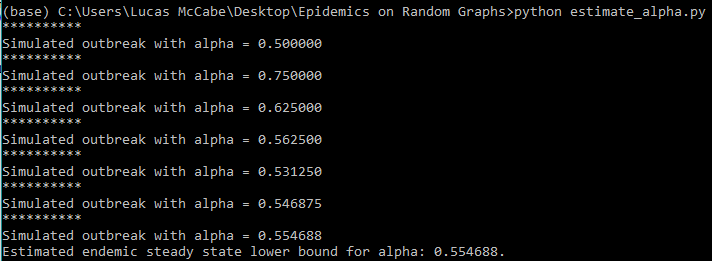
\includegraphics[width=8cm]{estimate_alpha_example.PNG}
	\caption{Sample output of \textit{estimate\_alpha}. Here, we show an example of the approach described in Algorithm 1 to find the endemic steady state-inducing lower bound for $\alpha$ with parameters $n=2000$, $p_{adj} = 0.1$, $p_{inf}=0.35$, $\tau = 4$, $\phi = 0.65$, $d = 1$.  }
	\centering
	\label{fig1}
\end{figure}

\section{Concluding Remarks}

In this paper, we introduce a framework for modeling disease outbreaks occurring on classical random graphs. Beginning with first principles, we use analytical methods to study contact processes in classical random graphs and derive results comparable to those found using traditional compartmental epidemiological approaches. We find that some results from dynamical systems modeling remain unchanged when reframing the disease model within a random graph framework. We conclude with a unique search and simulation method for indentifying linear vaccine rollout strategies that induce herd immunity.





\pagebreak

\section{Supplemental: Sample Code for $estimate\_I$}

\begin{minted}[mathescape, linenos]{python}
def estimate_I(t: int,
                n: int,
                p_adj: float,
                p_inf: float,
                t_rec: int) -> int:
    '''
    Recursively calculates the number of infected individuals
    in a random graph SIR model.
    
    Arguments
    	t: the time step.
    	n: the number of nodes to simulate.
    	p_adj: the probability of two nodes being connected.
    	p_inf: probability that an infected person will infect
                each of their connections during a time step.
    	t_rec: the number of time steps it takes for an infected
                individual to recover from an infection.
    '''
    if t == 0:
        return 1
    
    estimate = estimate_I(t-1,n,p_adj,p_inf,t_rec)\
                *(1+(n-estimate_I(t-1,n,p_adj,p_inf,t_rec)\
                         -estimate_R(t-1,n,p_adj,p_inf,t_rec))\
                         	*p_adj*p_inf\
                  - 1.0/t_rec)
    return max(estimate, 0)
\end{minted}

\pagebreak

\section{Supplemental: Sample Code for $estimate\_R$}

\begin{minted}[mathescape, linenos]{python}  
def estimate_R(t: int,
                n: int,
                p_adj: float,
                p_inf: float,
                t_rec: int) -> int:
    '''
    Recursively calculates the number of recovered individuals
    in a random graph SIR model.
    
    Arguments
    	t: the time step.
    	n: the number of nodes to simulate.
    	p_adj: the probability of two nodes being connected.
    	p_inf: probability that an infected person will infect
                each of their connections during a time step.
    	t_rec: the number of time steps it takes for an infected
                individual to recover from an infection.
    '''
    if t==0:
        return 0
    
    estimate = estimate_R(t-1,n,p_adj,p_inf,t_rec)\
                +(estimate_I(t-1,n,p_adj,p_inf,t_rec)/t_rec)
    return min(estimate, n)
\end{minted}

\pagebreak

\section{Supplemental: Sample Code for the Virus Class}

\begin{minted}[mathescape, linenos]{python}
class Virus():
    def __init__(self,
                p_infect: float = 0.1,
                t_recover: float = 1):
        '''
        Constructor for the Virus class.

        Arguments:
            p_infect: probability that an infected person will infect their
                partner during an encounter.
            t_recover: the average number of time steps it takes for an infected
                individual to recover from an infection.
        Raises:
            ValueError: if p_infect is not in [0,1]
            ValueError: if t_recover is not in [0,inf)
        '''
        if 0<=p_infect<=1:
            self.p_infect = p_infect
        else:
            raise ValueError('p_infect must be between 0 and 1.')

        if 0<=t_recover:
            self.t_recover = t_recover
        else:
            raise ValueError('t_recover must be at least 0.')

        #p_recover is the parameter estimate of a geometric random variable
        #with E[Geo(p)]=t_recover
        self.p_recover = 1.0/t_recover
\end{minted}

\pagebreak

\section{Supplemental: Sample Code for the Vaccine Class}

\begin{minted}[mathescape, linenos]{python}
class Vaccine():
    def __init__(self,
                effectiveness: float = 0.5,
                rollout: str = 'immediate',
                prevalence: float = 0,
                delay: float = 0,
                rate: float = 0):
        '''
        Constructor for the Vaccine class.

        Arguments:
            effectiveness: Vaccine effectiveness. Describes fraction of
                potential transmissions that are avoided thanks to the vaccine.
            rollout: Describes rollout. Two varieties are currently supported:
                'immediate' - After delay, vaccine immediately has specified
                    prevalence.
                'linear' - Linear rollout occurs with specified rate.
            prevalence: Fraction of nodes who have the vaccine. If rollout is
                linear, this varies.
            delay: Number of time steps before rollout begins.
            rate: Rate parameter for linear rollout.
        '''
        if 0<=effectiveness<=1:
            self.effectiveness = effectiveness
        else:
            raise ValueError('effectiveness must be between 0 and 1.')

        if rollout.lower() in ['immediate', 'linear']:
            self.rollout = rollout.lower()
        else:
            raise ValueError('Invalid rollout provided.')

        if 0<=prevalence<=1:
            self.prevalence = prevalence
        else:
            raise ValueError('prevalence must be between 0 and 1.')

        if delay >= 0 and int(delay)==delay:
            self.delay = delay
        else:
            raise ValueError('delay must be an integer at least zero.')

        if 0<=rate<=1:
            self.rate = rate
        else:
            raise ValueError('rate must be between 0 and 1.')

        if self.rollout == 'linear' and prevalence != 0:
            raise ValueError('prevalence must start at 0 with variable rollout.')

\end{minted}

\pagebreak

\section{Supplemental: Sample Code for the Experiment Class}

\begin{minted}[mathescape, linenos]{python}
import numpy as np
import random
import datetime
import math
import copy
from RG_SIR.virus import Virus
from RG_SIR.vaccine import Vaccine

class Experiment():
    '''
    Simulates an SIR disease model spreading over a classical random graph.

    General framework:
        -Begin with a classical random graph G(population, p_adjacent), with one
        node having a Virus(p_infect, t_recover).
        -During a time step, each infected node spreads the virus to each
        of its connected nodes with probability p_infect. For clarity, the
        expected number of nodes and infected node v will infect in a given time
        step is given by p_infect*degree(v).
        -At each time step, each infected node recovers with probability
        self.virus.p_recover, which is set to the maximum likelihood estimate
        of a parameter p for a geometric random variable whereby
        E[Geo(p)] = self.t_recover.
    '''

    def __init__(self,
                population: int = 100,
                p_adjacent: float = 0.1,
                virus: object = Virus(p_infect = 0.1,
                                        t_recover = 1),
                vaccine: object = Vaccine(effectiveness = 0.5,
                                            rollout = 'immediate',
                                            prevalence = 0,
                                            delay = 0,
                                            rate = 0),
                max_threshold: float = 1.0
                ):
        '''
        Constructor for the Experiment class. Initializes world for
        experimentation.

        Arguments:
            population: the number of nodes to simulate.
                Corresponds to the n in G(n,p).
            p_adjacent: the probability of two nodes being connected.
                Corresponds to the p in G(n,p).
            p_infect: probability that an infected person will infect each of
                their connections during a time step.
                For clarity, the expected number of nodes and infected node v
                will infect in a given time step is given by p_infect*degree(v).
            t_recover: the average number of time steps it takes for an infected
                individual to recover from an infection.
            max_threshold: the simulation halts if at least this fraction of
                the population becomes infected.
        Raises:
            ValueError: if population is not >0.
            ValueError: if p_adjacent is not in [0,1].
        '''
        if population <= 0:
            raise ValueError('Cannot have negative or zero population.')
        elif max_threshold < 0 or max_threshold > 1:
            raise ValueError('max_threshold must be between 0 and 1.')
        elif p_adjacent < 0 or p_adjacent > 1:
            raise ValueError('Invalid probability for p_adjacent.')
        else:
            self.population = population
            self.p_adjacent = p_adjacent
            self.virus = virus
            self.vaccine = vaccine
            self.adjacency = self.init_adjacency()
            self.infected = self.init_infected()
            self.immune = self.init_immune()
            self.vaccinated = self.init_vaccinated()
            self.time_step = 0
            self.newly_infected = 1
            self.max_threshold = max_threshold

            #experiment history:
            self.infected_history = [1]
            self.immune_history = [0]


    def init_adjacency(self):
        '''
        Initializes adjacency matrix.

        Creates a square matrix of size population whose lower triangular
        values are drawn from a binomial distribution with probability
        p_adjacent. Matrix is then made symmetric with a zero diagonal.
        '''
        adjacency = np.random.binomial(1,
                                    self.p_adjacent,
                                    (self.population, self.population)
                                    )
        adjacency -= np.triu(adjacency) #makes upper triangle and diagonal zero
        adjacency += adjacency.T #makes upper triangle=lower triangle for symmetry
        return adjacency

    def init_infected(self):
        '''
        Initializes array describing infected nodes. At initialization, this is a
        one-dimensional array of length population with zeros everywhere except
        at one node (one infected node in the population).

        A value of zero indicates an uninfected node, and nonzero value
        indicates an infected node.
        '''
        infected = np.zeros(self.population)
        infected[random.randint(0, self.population-1)] = 1
        return infected

    def init_immune(self):
        '''
        Initializes array describing immune nodes. At initialization, this is a
        one-dimensional array of length population with zeros everywhere (at
        first, zero nodes have immunity). After an infected node recovers, they
        are designated immune and can neither catch nor pass on the virus.
        '''
        immune = np.zeros(self.population)
        return immune

    def init_vaccinated(self):
        '''
        Initializes array describing vaccinated nodes. This is used to track
        vaccine rollout.
        '''
        if self.vaccine.rollout == 'immediate':
            #a fraction self.vaccine.prevalence of all nodes are randomly
            #selected to receive the vaccine
            vaccinated = np.zeros(self.population)
            vaccinated[:int(self.vaccine.prevalence*self.population)] = 1
            np.random.shuffle(vaccinated)
        if self.vaccine.rollout == 'linear':
            #if the rollout is linear, the initial vaccine prevalence is zero
            vaccinated = np.zeros(self.population)

        return vaccinated

    def count_infected(self):
        '''
        Returns the number of infected individuals.
        '''
        return np.count_nonzero(self.infected)

    def count_immune(self):
        '''
        Returns the number of recovered/naturally immune individuals.
        '''
        return np.count_nonzero(self.immune)

    def count_vaccinated(self):
        '''
        Returns the number of vaccinated individuals.
        '''
        return np.count_nonzero(self.vaccinated)

    def propagate_virus(self):
        '''
        Each infected node spreads the virus to each
        of its connected nodes with probability p_infect. For clarity, the
        expected number of nodes and infected node v will infect in a given time
        step is given by p_infect*degree(v).
        '''
        updated_infected = copy.deepcopy(self.infected)

        for i in range(self.population):
            if self.infected[i] == 1:
                #virus can only be spread from infected node
                for j in range(self.population):
                    #iterates adjacency row for node i
                    if (self.adjacency[i][j] == 1 and
                        random.random()<=self.virus.p_infect and
                        self.infected[j] == 0 and
                        self.immune[j] == 0):
                        #contact with an infected node occurs, opening the
                        #POSSIBILITY of transmission
                        #transmission cannot occur when potential recipient is
                        #(naturally) immune (e.g. recovered)
                        if (self.vaccinated[j] == 1 and
                            random.random()<=self.vaccine.effectiveness):
                            #transmission is avoided with probability
                            #self.vaccine.effectiveness in the case of
                            #vaccinated recipient
                            continue
                        updated_infected[j] = 1
        self.newly_infected = np.sum(updated_infected - self.infected)
        self.infected = updated_infected

        return None

    def update_infected(self):
        '''
        Each infected node recovers with probability self.virus.p_recover.
        '''
        for i in np.where(self.infected == 1)[0]:
            if random.random() <= self.virus.p_recover:
                self.infected[i] = 0
                self.immune[i] = 1
        return None

    def update_vaccinated(self):
        '''

        Raises:
            NotImplementedError for unimplemented rollouts. Shouldn't really
                happen.
        '''
        if self.vaccine.rollout == 'immediate':
            return None
        if self.vaccine.rollout == 'linear':
            if self.time_step >= self.vaccine.delay:
                #self.vaccine.rate*self.population is the number of new nodes
                #that become vaccinated each time step.
                if len(np.where(self.vaccinated == 0)[0]) <= \
                                            self.vaccine.rate*self.population:
                    #If there are fewer than self.vaccine.rate*self.population
                    #unvaccinated nodes remaining, all nodes become vaccinated.
                    self.vaccinated = np.ones(self.population)
                else:
                    self.vaccinated[random.sample(
                                    list(np.where(self.vaccinated == 0)[0]),
                                    int(self.vaccine.rate*self.population))] = 1
        else:
            raise NotImplementedError

    def update_history(self):
        '''
        Updates experiment history for tracking.
        '''
        self.infected_history.append(self.count_infected())
        self.immune_history.append(self.count_immune())
        return None

    def simulate_step(self):
        '''
        Simulates a single simulation time step. Three events occur:
        1. Virus is propagated by infected nodes.
        2. Infected nodes become one step closer to recovery.
        3. Newly-recovered nodes become immune.

        If the vaccine rollout is not immediate, a fourth event occurs:
        4. The number of nodes vaccinated updates according to the defined
        rollout strategy.
        '''
        self.propagate_virus() #handles event 3
        if self.time_step != 0:
            self.update_infected() #handles events 2 and 3
        self.update_vaccinated() #handles event 4
        self.update_history() #updates history for tracking experiment
        self.time_step += 1
        return None

    def calculate_ever_infected(self):
        '''
        Returns the total number of nodes have ever had the virus. This is
        the sum of count(nodes who currently have the virus) and
        count(nodes who are now immune).
        '''
        ever_infected = np.add(self.infected, self.immune)
        np.place(ever_infected, ever_infected>0, 1)
        return np.sum(ever_infected)

    def print_progress(self):
        '''
        Prints interesting progress metrics for each time step.
        '''
        print('**********')
        print('Time step: %d:' %self.time_step)
        print('Newly Infected: %d' %self.newly_infected)
        print('Max Infected At Once: %d' %max(self.infected_history))
        print('Total Infected Now: %d' %self.count_infected())
        print('Total Vaccinated Now: %d' %self.count_vaccinated())
        print('Total Recovered/Immune Now: %d' %self.count_immune())

    def run_experiment(self, show_progress: bool = False):
        '''
        Runs an experiment. Experiment stops when either one of:
            1. The entire population is infected.
            2. The entire population has recovered.

        Arguments:
            show_progress: If True, prints some progress metrics.
        Returns:
            None
        '''
        while (0 < self.count_infected() < self.population*self.max_threshold):
            if show_progress:
                self.print_progress()
            self.simulate_step()
        if show_progress:
            self.print_progress()
        print('**********')
        return None

    def save_experiment_results(self):
        '''
        Saves experiment history/results to a text file. The file contains six
        lines, population as follows:
            -population
            -p_adjacent
            -p_infect
            -t_recover
            -max number infected in any single time step
            -total number infected across the experiment
            -infected_history
            -immune_history
        '''
        experiment_id = str(datetime.datetime.now()).replace(' ','_')
        for ch in ['-', ':', '.']:
            experiment_id = experiment_id.replace(ch, '')

        with open('Trials/Trial_' + experiment_id + '.txt', 'w') as output:
            for param in [self.population,
                        self.p_adjacent,
                        self.virus.p_infect,
                        self.virus.t_recover,
                        max(self.infected_history),
                        self.calculate_ever_infected()]:
                output.write('%s\n' %param)
            for i in range(self.time_step):
                output.write('%s ' %self.infected_history[i])
            output.write('\n')
            for i in range(self.time_step):
                output.write('%s ' %self.immune_history[i])

        output.close()
        return None

\end{minted}

\pagebreak

\section{Supplemental: Sample Code for \textit{estimate\_alpha}}

\begin{minted}[mathescape, linenos]{python}

r"""
Sample script exhibiting a binary search and simulation for estimating the
endemic steady state-inducing lower bound for alpha (rollout rate).

Intended for demonstration purposes only. Simply run the script directly from
the command line.

Example Usage:
>>> python estimate_alpha.py
**********
Simulated outbreak with alpha = 0.500000
**********
Simulated outbreak with alpha = 0.750000
**********
Simulated outbreak with alpha = 0.625000
**********
Simulated outbreak with alpha = 0.562500
**********
Simulated outbreak with alpha = 0.531250
**********
Simulated outbreak with alpha = 0.546875
**********
Simulated outbreak with alpha = 0.554688
Estimated endemic steady state lower bound for alpha: 0.554688.
"""

from RG_SIR.experiment import Experiment
from RG_SIR.virus import Virus
from RG_SIR.vaccine import Vaccine

#ADJUST PARAMS HERE-----
population = 2000
p_adjacent = 0.1
p_infect = 0.35
t_recover = 4
effectiveness = 0.65
rollout = 'linear'
prevalence = 0
delay = 1

stop_within = 0.01
#-------

alpha_high = 1.0
alpha_low = 0.0

while (abs(alpha_high-alpha_low) >= stop_within):
    alpha = (alpha_high+alpha_low)/2

    experiment = Experiment(population = population,
                            p_adjacent = p_adjacent,
                            virus = Virus(p_infect=p_infect,
                                        t_recover = t_recover),
                            vaccine = Vaccine(effectiveness = effectiveness,
                                        rollout = rollout,
                                        prevalence = prevalence,
                                        delay = delay,
                                        rate = alpha)
                            )

    experiment.run_experiment(show_progress = False)

    print('Simulated outbreak with alpha = %f' %alpha)
    #print(max(experiment.infected_history))

    if max(experiment.infected_history) < (1 - (1/t_recover))*0.925*population:
        alpha_high = alpha
    else:
        alpha_low = alpha


print('Estimated endemic steady state lower bound for alpha: %f.' %alpha)

\end{minted}


\end{document}
